\documentclass[11pt,a4paper]{article}
\usepackage[utf8]{inputenc}
\usepackage[T1]{fontenc}
\usepackage[english]{babel}
\usepackage[margin=2.1cm]{geometry}
\usepackage{booktabs,array,tabularx}
\usepackage{xcolor}
\usepackage{graphicx}
\usepackage{pgfplots}
\pgfplotsset{compat=1.17}
\PassOptionsToPackage{hyphens}{url}
\usepackage[hidelinks]{hyperref}
\usepackage{enumitem}
\setlist{nosep,leftmargin=1.4em}
\emergencystretch=3em

\definecolor{impl}{HTML}{3B6EA8}
\definecolor{rev}{HTML}{8FB3DA}
\definecolor{waste}{HTML}{C0504D}

\title{Sweatshop on P-Chess: lane \texttt{mvp}\\\large CI test job, themes and sounds, the engine fetch script (CI-001, UI-003, BOT-001) and the Windows export (CI-002, parked); day lineup, then Opus 5.5}
\author{Foreman, session \texttt{sweatshop/mvp/2026-10-24-1310}}
\date{24 October 2026}

\begin{document}
\maketitle

\section*{Summary}

Lane \texttt{mvp} ran in the clone \path{.artifacts-build/lanes/mvp}, from \texttt{main} at
\texttt{66cd0ab}. It holds the \texttt{Review: human} tickets, and every queued ticket of the
other lanes waited on one of them, BOT-001. Two launches: 13:10 (pid 18032, default day
lineup: stage 2 \texttt{gpt-6.1-sol high}, stage 3 and hard \texttt{gpt-6.1-sol xhigh}, on
Codex; launched by the coordinating session and adopted by this foreman at 13:12; paused with
\texttt{STOP} at 14:09) and 14:11 (pid 5808, \texttt{-Models 'stage 2 opus-5.5 high, hard
opus-5.5 xhigh, stage 3 opus-5.5 xhigh'} at Bruno's request; ended 14:16 with ``Nothing
runnable'').

\begin{itemize}
  \item \textbf{Produced:} \textbf{3 tickets approved and merged on the session} PR
        \href{https://github.com/Laginho/P-Chess/pull/5}{\#5}: CI-001, UI-003, BOT-001, all
        \texttt{Review: human}, \texttt{Verdict: Approve}. CI-002 is implemented and reviewed
        on \texttt{ci-002} but parked \texttt{blocked}, by contract, outside the session.
  \item \textbf{Cost:} \textbf{\$8.07} at API list price over 9 stages, all priced:
        \texttt{gpt-6.1-sol high} \$3.50 (1 point of the weekly Codex quota),
        \texttt{gpt-6.1-sol xhigh} \$3.14 (2 points), \texttt{opus-5.5 xhigh} \$1.44
        (\texttt{--}).
  \item \textbf{What went wrong:} criterion 6 of BOT-001 asked to compare the pinned hashes
        with Bruno's \path{engine/} copies, which do not exist on this machine. The first
        review held the ticket for Bruno; once he accepted the official GitHub artifacts as
        the baseline, the re-review merged in 5 minutes, but the driver then refused the
        reused gate receipt because its own CI-002 parking note had changed another ticket's
        file. The foreman reran the gate (81/81) and restored \texttt{done}.
  \item \textbf{Provisional verdict:} the day lineup did the work cleanly: four first-attempt
        handoffs, zero review findings, zero reopens. Everything that cost time was the
        contract (a reference that never existed) or the driver (receipt check, re-entry
        after a held review), not the models.
\end{itemize}

\section*{What was done}

\textbf{CI-001}: every push now runs the test suite on GitHub Actions, on Ubuntu with Godot
4.7.2 checked against its published SHA-256, with exactly the local gate command, so a red
test shows on the branch before review. Main file \path{.github/workflows/ci.yml}. Proof: a
green push run (78/78) and, on the session tip \texttt{0b05c75}, run
\href{https://github.com/Laginho/P-Chess/actions/runs/40115493475}{40115493475}, 81/81.

\textbf{UI-003}: the board can be themed. \path{ui/theme_loader.gd} loads a board
\texttt{theme.json}, the twelve cburnett piece SVGs and one OGG per sound event from
\texttt{res://themes/} or \texttt{user://themes/}; \path{ui/sound_player.gd} plays move,
capture, castle, check, promotion, game start and game end. The four free Lichess sets
(\texttt{sfx}, \texttt{nes}, \texttt{piano}, \texttt{futuristic}) are bundled; \texttt{sfx}
is the default until Bruno picks one by ear.

\textbf{BOT-001}: \path{scripts/fetch-engine.ps1} (Windows PowerShell 5.1) downloads Lc0
v0.32.1 CPU dnnl and the nine Maia v1.0 nets into \path{engine/}, checks 20 pinned SHA-256
hashes (the zip, its ten entries, nine nets), deletes a file and exits 1 on any mismatch, and
skips files that already verify. \path{docs/THIRD_PARTY.md} names both GPL-3 projects and
their tags. Criterion 6 was rewritten from Bruno's decision: the hashes come from the
official downloads; the Lc0 zip matches GitHub's published digest; Maia publishes none.

\textbf{CI-002} (not integrated): \path{export_presets.cfg} and a second CI job export the
Windows build and upload it as an artifact without \path{engine/} (49 theme assets verified
in the package, run
\href{https://github.com/Laginho/P-Chess/actions/runs/40113823385}{40113823385}). It waits on
BOT-002 and BOT-004 for the missing-engine message (criterion 5) and on a human listening to
the move sound (criterion 6).

\section*{Timeline}

\begin{tabularx}{\linewidth}{@{}lX@{}}
\toprule
13:10 & Driver launched by the coordinating session, pid 18032, day lineup. \\
13:12 & Adopted by this foreman. Bruno's \path{engine/} folder not found on disk. \\
13:15--13:35 & CI-001 and UI-003 implemented and merged on the session, 0 findings. CI-001's stage 2 pushed \texttt{ci-001} to \texttt{origin} for its Actions proof. \\
13:47 & BOT-001 to review. Foreman audit: downloads only from the two official releases; zip hash equals GitHub's digest. \\
13:51 & BOT-001 review: 0 findings, held as \emph{Needs your call}; proxy escalated criterion 6. \\
13:58 & Bruno (relayed): accept the official artifacts as the baseline. \\
14:04--14:09 & CI-002 implemented (pushed \texttt{ci-002}) and reviewed, parked by contract. \\
14:08 & Bruno (relayed): stop after this ticket, switch to the Opus lineup. \texttt{STOP} honoured at 14:09; PR \#5 opened. \\
14:10 & Foreman: session revert of the parking commit (\texttt{91627ec}), decision folded into criterion 6 on \texttt{BOT-001} (\texttt{d0b0787}). \\
14:11--14:16 & Relaunch, pid 5808. BOT-001 re-review merged and closed (\texttt{83b8d00}, \texttt{3f5e335}); driver parked it for a stale receipt (\texttt{5225e25}). \\
14:18 & Foreman: revert (\texttt{2583e7f}), gate rerun 81/81, receipt line updated (\texttt{0b05c75}). Nothing runnable: BOT-007 waits on BOT-006, CI-003 on CI-002. \\
\bottomrule
\end{tabularx}

\section*{Per stage}

{\small
\begin{tabularx}{\linewidth}{@{}llllrrrrrX@{}}
\toprule
When & Ticket & Stage & Model & Min & In & Cache & Out & Cost & Outcome \\
\midrule
13:15 & CI-001 & impl & sol high & 5 & 1.3M & 96\% & 6k & 0.42 & to-review \\
13:19 & CI-001 & review & sol xhigh & 4 & 1.5M & 92\% & 10k & 0.64 & merged \\
13:31 & UI-003 & impl & sol high & 12 & 2.8M & 96\% & 20k & 0.95 & to-review \\
13:35 & UI-003 & review & sol xhigh & 4 & 2.2M & 91\% & 13k & 0.90 & merged \\
13:47 & BOT-001 & impl & sol high & 12 & 2.9M & 96\% & 22k & 1.03 & to-review \\
13:51 & BOT-001 & review & sol xhigh & 5 & 1.5M & 88\% & 15k & 0.76 & held for Bruno \\
14:04 & CI-002 & impl & sol high & 12 & 3.4M & 97\% & 21k & 1.10 & to-review \\
14:09 & CI-002 & review & sol xhigh & 5 & 1.8M & 90\% & 13k & 0.84 & parked (contract) \\
14:16 & BOT-001 & review & opus xhigh & 5 & 2.7M & 95\% & 31k & 1.44 & merged$^{*}$ \\
\midrule
 & & & & 64 & 20.1M & & 151k & 8.07 & \\
\bottomrule
\end{tabularx}
}

\smallskip
{\small $^{*}$ The run-log row reads \texttt{failed (incomplete handoff), blocked}: the review
merged and closed the ticket, and the driver then parked it over the receipt check. The row
is left as logged; what happened is above.}

\begin{center}
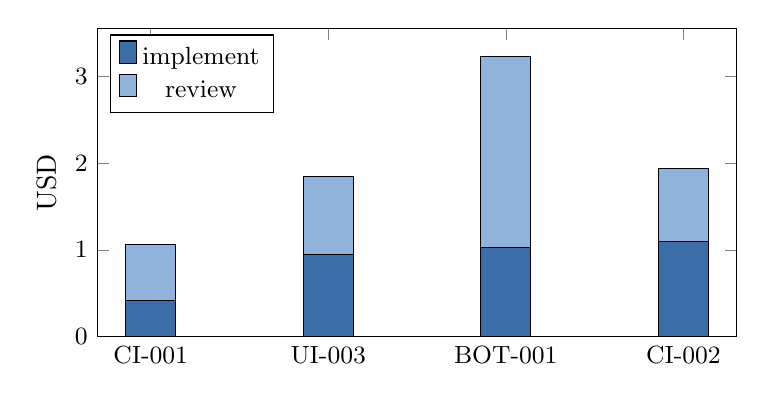
\begin{tikzpicture}
\begin{axis}[ybar stacked, bar width=18pt, width=0.8\linewidth, height=5.5cm,
  symbolic x coords={CI-001,UI-003,BOT-001,CI-002},
  xtick=data, ylabel={USD}, ymin=0, legend style={at={(0.02,0.98)},anchor=north west,font=\small},
  tick label style={font=\small}]
\addplot[fill=impl] coordinates {(CI-001,0.42) (UI-003,0.95) (BOT-001,1.03) (CI-002,1.10)};
\addplot[fill=rev] coordinates {(CI-001,0.64) (UI-003,0.90) (BOT-001,2.20) (CI-002,0.84)};
\legend{implement, review}
\end{axis}
\end{tikzpicture}
\end{center}

No attempt was lost. BOT-001's second review (\$1.44) is the price of a criterion that named a
reference nobody had: the first review could only hold it. Input is 88--97\% cache reads.

\section*{Comparison with previous runs}

Earlier lanes today, from \texttt{run-log.md}: \texttt{skeleton} (CORE-001, \$5.61),
\texttt{bot} (BOT-003, \$4.87 before its two reworks), \texttt{core} (\$7.20 per approved
ticket). Lane \texttt{mvp}: \$2.69 per approved ticket (\$8.07 over 3, CI-002's \$1.94
included). These tickets were small (a workflow, a loader, a script), and the day lineup ran
4--12 minute implementations against 3--14 for Opus overnight.

\section*{Observations per model}

\begin{itemize}
  \item \textbf{gpt-6.1-sol high (stage 2)}: 4 runs, 4 to review on the first attempt, 5--12
        minutes, \$0.42--\$1.10. Every handoff disclosed what it could not prove (UI-003's
        listening test, BOT-001's missing reference, CI-002's dependency). On both CI tickets
        it pushed its ticket branch to \texttt{origin} to get the Actions run the ticket
        demands; the foreman rule forbids pushing ticket branches.
  \item \textbf{gpt-6.1-sol xhigh (review)}: 4 reviews, 0 findings, 0 reopens. It held BOT-001
        and CI-002 instead of approving past an open condition, and checked the Lc0 digest
        and Godot template hashes against upstream itself.
  \item \textbf{opus-5.5 xhigh (review)}: 1 re-review, 5 minutes. It reviewed only the
        post-review delta (ticket text), reused the gate receipt because production was
        unchanged, and dismissed one wrong Standards finding from its own subagent.
\end{itemize}

\section*{Driver and runtime issues}

\begin{enumerate}
  \item \textbf{The driver's own note invalidates its receipt check.} At \texttt{done} the
        driver diffs the tested commit against the session, excluding only the ticket and its
        ledger. Its CI-002 parking note (\texttt{9f61f41}) landed on the session in between,
        so BOT-001's valid merge was parked. Third time today (BOT-002, UI-002, BOT-001).
  \item \textbf{No re-entry for a held review.} After a human answers a \emph{Needs your
        call}, the session copy says \texttt{blocked}, which the driver honours over the
        branch. The foreman had to revert the parking commit by hand so the driver would read
        the branch's \texttt{to-review}.
  \item \textbf{CI tickets need a push.} CI-001 and CI-002 can only prove themselves on
        Actions; stage 2 pushed \texttt{ci-001} and \texttt{ci-002}. Both remote branches are
        still on \texttt{origin}.
  \item \textbf{Run-log outcome mislabels the last BOT-001 review} (above).
\end{enumerate}

\section*{Recommendations}

\begin{enumerate}
  \item Exclude every \path{.scratch/*/issues/*.md} from the ``code changed after gate'' diff:
        ticket text is not production. Rests on three parked merges today, no scoreboard row.
  \item Give the driver an \texttt{-Answer <ID>} (or document the revert) for a held review:
        drop the session's parking commit and let the branch's stage lead.
  \item Say in \texttt{ticket-flow} how a CI ticket gets its Actions proof: push the ticket
        branch and delete it at merge, or run the workflow on the session branch.
  \item Write criteria that name a human's local files only after checking they exist;
        BOT-001's criterion 6 cost one review and a relaunch.
  \item Keep \texttt{gpt-6.1-sol high} $\rightarrow$ \texttt{gpt-6.1-sol xhigh} for small
        \texttt{Review: human} tickets: scoreboard row 89 reviews, 13\% reopen, 12\% S2 rate,
        the lowest S2 rate among pairs with more than 10 reviews.
\end{enumerate}

\section*{Human debt and proxy decisions}

No \texttt{Débito humano:} lines this run. \texttt{Proxy decided} lines, all by the
\texttt{gpt-6-astra high} fallback:

\begin{itemize}
  \item \textbf{BOT-001}: ``Proceed with stage 2 using hashes computed from official upstream
        downloads; preserve comparison with Bruno's copies as an explicit human integration
        gate.'' The review's \texttt{Proxy escalated} line sent criterion 6 to Bruno, who
        decided: official GitHub artifacts are the baseline.
  \item \textbf{CI-002}: ``implement and independently review the CI-002 exporter now
        \ldots{} preserve criterion 5 as pending until BOT-002 and BOT-004 provide the visible
        missing-engine flow''; and at review, ``record the completed CI-002 review with
        Stage: blocked on ci-002, retaining the implementation without session
        integration''.
\end{itemize}

\section*{Reopen attribution}

No reopened review this run, and no merging review authored a fix: no rows added to
\path{.scratch/reopen-attribution.md}. PR \#5 has one review, Copilot's, which did not run
(quota); no session-review, release-audit or post-release finding.

\section*{Scoreboard}

\texttt{scoreboard.ps1} over P-Chess (main checkout, log merged and copied back), ClassyCall,
EasyMath, PhysiSyst, SIGAA-ME, SynchroNice and slip. Rows that moved since the
\texttt{core} report: \texttt{gpt-6.1-sol high} $\rightarrow$ \texttt{gpt-6.1-sol xhigh} 87
$\rightarrow$ 89 reviews, 12 reopened (rate 14\% $\rightarrow$ 13\%), from this run's two
merges (the held reviews of BOT-001 and CI-002 do not count as reviews with a verdict);
\texttt{opus-5.5 high} $\rightarrow$ \texttt{opus-5.5 xhigh} 4 $\rightarrow$ 6 reviews and
\texttt{opus-5.5 xhigh} $\rightarrow$ \texttt{opus-5.5 xhigh} 3 $\rightarrow$ 5, both from
other lanes. Opus pairs remain under 10 reviews: anecdotes.

{\small
\begin{tabular}{@{}llrrrrr@{}}
\toprule
Implementer & Reviewer & Reviews & Reopened & Rate & S2 & S2 rate \\
\midrule
gpt-6.1-sol high & gpt-6.1-sol xhigh & 89 & 12 & 13\% & 11 & 12\% \\
gpt-6.1-sol high & gpt-6.1-sol max & 94 & 21 & 22\% & 20 & 21\% \\
opus-5.5 high & opus-5.5 xhigh & 6 & 2 & 33\% & 2 & 33\% \\
opus-5.5 xhigh & opus-5.5 xhigh & 5 & 0 & 0\% & 0 & 0\% \\
\bottomrule
\end{tabular}
}

\medskip
Implementers: \texttt{gpt-6.1-sol high} 216 runs, 187 to review, 8 failed, 21 asked, median
20 min, \$369.21. Interventions across repos: 22 human rescues, 46 automatic recoveries, 4
routine approvals, 27 \texttt{gpt-6-astra high, fallback} proxy decisions, 15 Opus. This
run's five intervention rows are committed on \texttt{main} with this report; the printout
above was taken from the main checkout before that commit, so they are not in it. Full
printout: the foreman's scratch output.

\section*{Pending for the human}

\begin{enumerate}
  \item Review and merge PR \#5 (CI-001, UI-003, BOT-001, all \texttt{Review: human}). Every
        queued ticket of the other lanes waits on BOT-001 reaching \texttt{main}.
  \item UI-003: listen to the four sound sets and name the default (\texttt{sfx} for now).
  \item CI-002: after BOT-002 and BOT-004 are integrated, a fresh Actions artifact must show
        the fetch-script message on Windows, and someone must hear the move sound.
  \item Delete \texttt{origin/ci-001} and \texttt{origin/ci-002}.
\end{enumerate}

\end{document}
